
\documentclass[twoside,twocolumn]{article}

\usepackage{blindtext} % Package to generate dummy text throughout this template 

\usepackage[sc]{mathpazo} % Use the Palatino font
\usepackage[T1]{fontenc} % Use 8-bit encoding that has 256 glyphs
\linespread{1.05} % Line spacing - Palatino needs more space between lines
\usepackage{microtype} % Slightly tweak font spacing for aesthetics

\usepackage[english]{babel} % Language hyphenation and typographical rules

\usepackage[margin=0.5in,top=15mm,columnsep=10pt]{geometry} % Document margins
\usepackage[hang, small,labelfont=bf,up,textfont=it,up]{caption} % Custom captions under/above floats in tables or figures
\usepackage{booktabs} % Horizontal rules in tables

\usepackage{lettrine} % The lettrine is the first enlarged letter at the beginning of the text

\usepackage{enumitem} % Customized lists
\setlist[itemize]{noitemsep} % Make itemize lists more compact

\usepackage{abstract} % Allows abstract customization
\renewcommand{\abstractnamefont}{\normalfont\bfseries} % Set the "Abstract" text to bold
\renewcommand{\abstracttextfont}{\normalfont\small\itshape} % Set the abstract itself to small italic text

\usepackage{titlesec} % Allows customization of titles
\renewcommand\thesection{\Roman{section}} % Roman numerals for the sections
\renewcommand\thesubsection{\roman{subsection}} % roman numerals for subsections
\titleformat{\section}[block]{\large\scshape\centering}{\thesection.}{1em}{} % Change the look of the section titles
\titleformat{\subsection}[block]{\large}{\thesubsection.}{1em}{} % Change the look of the section titles

\usepackage{fancyhdr} % Headers and footers
\pagestyle{fancy} % All pages have headers and footers
\fancyhead{} % Blank out the default header
\fancyfoot{} % Blank out the default footer
\fancyhead[C]{MSc ACSE -6 Individual Assessment 2022 $\bullet$ Feb 2022 } % Custom header text
\fancyfoot[RO,LE]{\thepage} % Custom footer text

\usepackage{titling} % Customizing the title section

\usepackage{hyperref} % For hyperlinks in the PDF

\usepackage{graphicx} %package to manage images
\usepackage{subfigure}
\usepackage{caption}
\usepackage{subcaption}
\usepackage{booktabs}
\usepackage{float}

\usepackage[table,xcdraw]{xcolor}
\graphicspath{ {./images/} }
%----------------------------------------------------------------------------------------
%	TITLE SECTION
%----------------------------------------------------------------------------------------

\setlength{\droptitle}{-4\baselineskip} % Move the title up

\pretitle{\begin{center}\Huge\bfseries} % Article title formatting
\posttitle{\end{center}} % Article title closing formatting
\title{ANALYSIS REPORT FOR A 2-D WAVE SOLVER IMPLEMENTED IN C++ USING PARALLEL COMPUTING} % Article title
\author{%
\textsc{NIRANJANA SUNDARARAJAN}
}
\date{\today} % Leave empty to omit a date
\renewcommand{\maketitlehookd}{%
% \begin{abstract}
% \noindent \blindtext % Dummy abstract text - replace \blindtext with your abstract text
% \end{abstract}
}

%----------------------------------------------------------------------------------------

\begin{document}

% Print the title
\maketitle

%----------------------------------------------------------------------------------------
%	ARTICLE CONTENTS
%----------------------------------------------------------------------------------------
\lettrine[nindent=1em,lines=2]{T}he following report is based on the a scalable software designed to implement a 2-D Wave Solver using parallelising concepts from MPI. The software aims to solve a 2-D domain through the discretisation of its PDE in both time and space. The main input parameters include the duration of the run, the grid size and the boundary conditions(among others). There are three boundary conditions implemented for this software - Dirichlet, Neumann and Periodic and the user may pick from amongst these. The initial disturbance is by default to a single point type and can be further expanded to include multiple points or a sinusoidal wave. Finally, we have the post-processing and visualisations of these results in the form of animated gifs.\\
This report aims to highlight the findings and inferences of the performance of the code using data obtained from running this solver using the HPC resources, for different combination of nodes and cores. It will also briefly discuss the various design choices made while writing the code and the further improvements and optimizations, should this code be expanded in the future.

%------------------------------------------------
\section{Code Structure, Design Decisions and Optimisations}
The figure below shows all the source files that contain classes and their associated functions. The code is designed to be as modular as possible, keeping in mind OOPs principles in order to facilitate future scalability and extension in functionalities of each of the classes and.
\vspace{-4mm}
\begin{figure}[h]
\centering
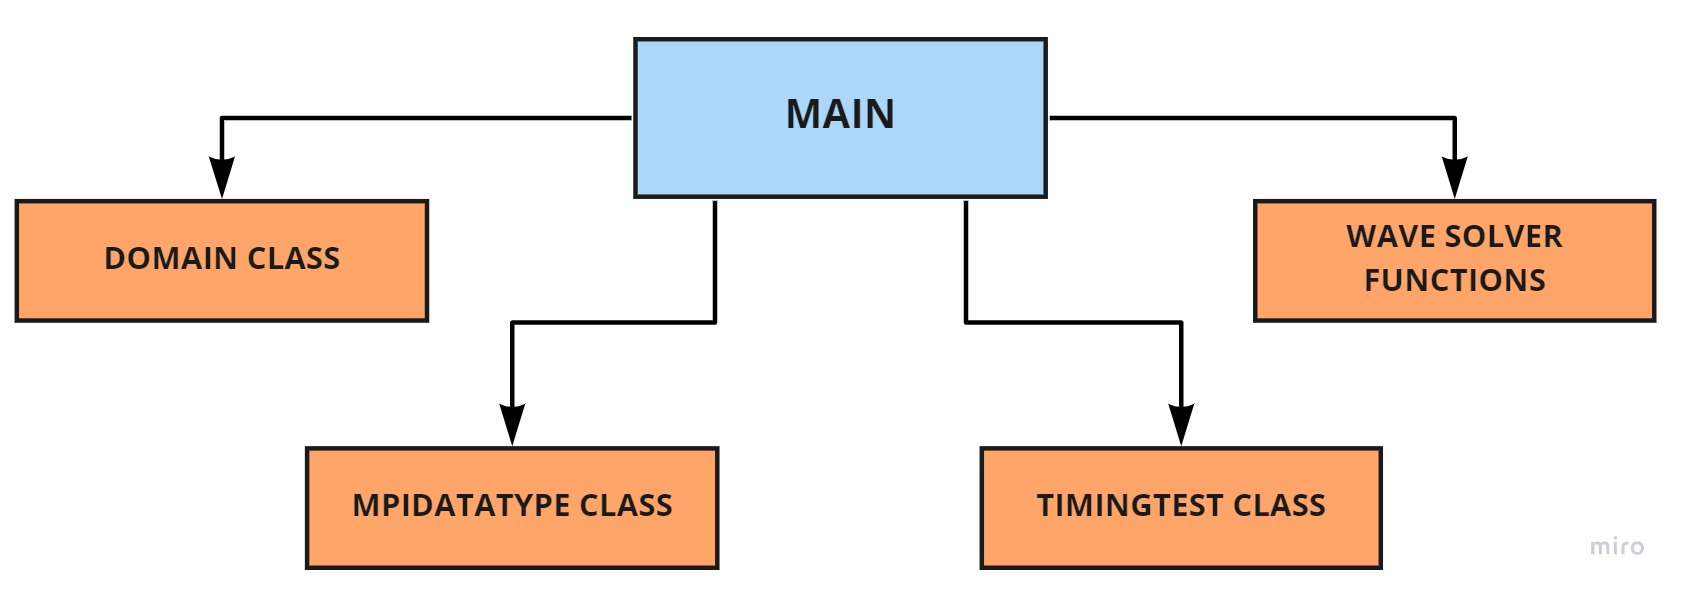
\includegraphics[height=3.5 cm\textwidth]{images/FileStructure.jpg}
\caption{Source Files and Classes Hierarchies}
\end{figure}

The code is structured keeping in mind an optimization for performance. The Domain class that is responsible for \textbf{domain decomposition} is implemented such that each processor only allocates enough memory to store its portion of the domain. Further the the grid is split between the processors in a way that the sub-domains are as close to square as possible to ensure maximum efficiency during MPI communications. \textbf{Workload balancing} was maintained such that all processes finish their tasks in similar times. This avoided the need to implement any costly synchronization efforts or barriers. \\
Since each process need only communicate with a subset of its neighbours, the eight MPI Datatypes were setup to allow for a \textbf{non-blocking type peer-to-peer communication} to ensure maximum scalability for all three boundary conditions.The receives were called before the send, and together in a single loop to further optimise for performance.\\
Only three time step values are stored and the \textbf{calculations are staged} such that the inner domain iteration is carried on while the code waits for the MPI communications to complete. This further improves performance of the code. Further, all loopings are carried out in \textbf{row major ordering} to reduce cache misses as much as possible. To avoid unnecessary time costs, the code also ensures to loop only over the region that is necessary for the time-stepping and not the whole sub-domain.\\
Each processes then writes it own file to output, depending on the boundary condition,into separate folders that are then ready for post-processing. Finally, the \textbf{Timing Test class} is one that serves two purposes  - first, to declare variables and functions that robustly measure performance of different sections of the code and second, to store timings from each of the processes for further analysis related to load balancing.
\vspace{-4mm}
\section{Performance Analysis : Introduction}
Using the performance profiler in visual studio showed that, as expected, the time-stepping function for the inner domain was the most expensive function(89\%), followed by read-write functions. A further breakdown of the code will allow us to analyse different functions using different domain sizes and cores used for parallelisation.\\

\textbf{Key Variables and Output Parameters} \\
The code was compiled and run on the HPCs for matrix inputs ranging from 100x100 to 1000x1000 for both the Dirichlet and the Neumann boundary conditions and from 500x500 - 1000x1000 for the periodic boundary condition. For the sake of comparative calculations, a set of serial outputs were also computed for each of these cases. Other parameters computed during the HPC calculations included(for a single process) :  \\
- Time spent to setup the domain \\
- Time spent to create MPI Data Types\\
- Time spent  to carry out MPI communications \\
- Time spent  to finish a set of inner iterations\\
- Time spent  to finish a set of edge iterations\\
- Total time for a processor \\
For clarity and ease of analysis, the code also outputs the simulation parameters including domain size, total number of processes used, the boundary type, the Tmax and the total iterations to reach Tmax. These will be useful for further analysis. An example of the outputs generated is illustrated in the figure below
\vspace{-4mm}
\begin{figure}[h]
\centering
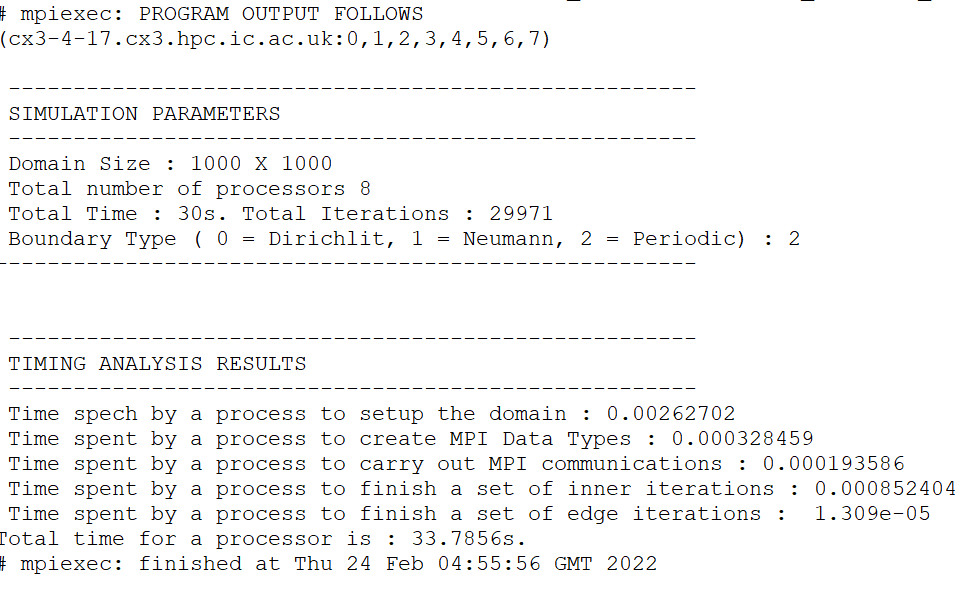
\includegraphics[height=5.5 cm\textwidth]{images/hpcoutput.png}
\caption{HPC Output: 1000x1000 Domain, Periodic Boundary Conditions}
\end{figure}

Using the data collected the following aspects are discussed in brief :\\
 - Speed Up Ratio, Parallel Efficiency and Amhdal's Law\\
 - Domain Decomposition Efficiency and Analysis\\
 - Affect of Domain Size and Shape on Performance\\
 - Efficiency of MPI Communications \\
 - Boundary Setup and Edge calculation Efficiencies \\
 - Comparisons
%----------------------------------------------------------------------------------------
\section{Speed Up Ratio, Parallel Efficiency and Limitations from Amdahl's Law}
The first general analysis carried out showed the variation of the speed up ratios over an increasing number of cores for Dirichlet and Neumann boundaries for a domain sizes ranging from 100x100 to 1000x1000. The figures below show the Speed Up ratios for the Neumann and Dirichlet boundary conditions for smaller(100x100 - 500x500) and larger (500x500 - 1000x1000) sizes.\\

\vspace{-4mm}
\begin{figure}[h]
\centering
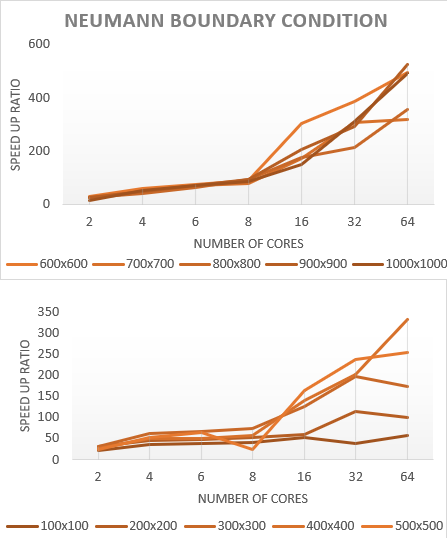
\includegraphics[height=10.5 cm\textwidth]{images/sppedupratios-neumann.png}
\caption{Variation of Speed Up ratios : Neumann Boundary Conditions}
\end{figure}

\begin{figure}[H]
\centering
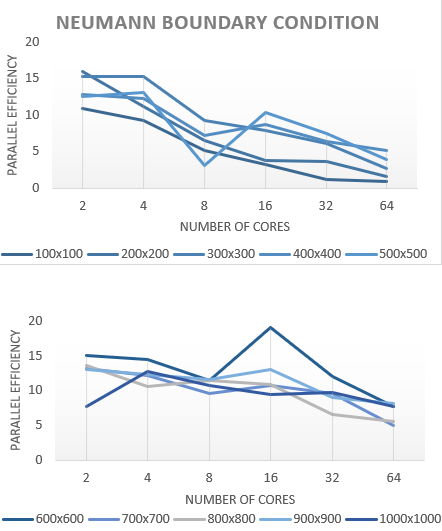
\includegraphics[height=10.5 cm\textwidth]{images/PARALLEL EFFICIENCY NEWMANN.png}
\caption{Parallel Efficiency Trends : Dirichlet boundary Conditions}
\end{figure}


As expected, we observe higher speed up ratios as the number of cores increase. However we can note that that a lot of the trends we expect are more pronounced in larger domains,to find the solution of which computational solvers such as the one designed are most optimal to use. 

\vspace{-4mm}
\begin{figure}[H]
\centering
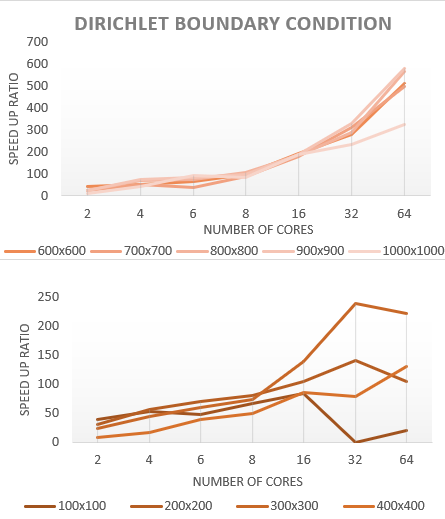
\includegraphics[height=10.5 cm\textwidth]{images/speedupratios - dirichlet.png}
\caption{Variation of Speed Up ratios : Dirichlet Boundary Conditions}
\end{figure}

\begin{figure}[H]
\centering
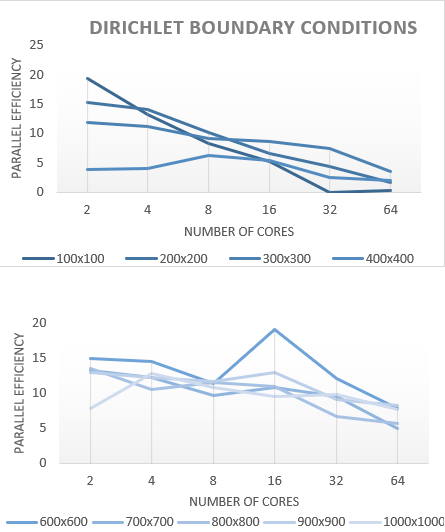
\includegraphics[height=10.5 cm\textwidth]{images/PARALLEL EFFICIENCY DIRICHELT.png}
\caption{Parallel Efficiency Trends : Dirichlet boundary Conditions}
\end{figure}
If we keep increasing the number of cores, after a point the effect of the speedup will be negligible. This is in line with \textbf{Amhdal's law} which limits the increase in the speedup ratios with increasing cores to (1/1-f) where f is fraction of code executing in parallel. This as seen in the figures below, the parallel efficiency drops with increase in the number of cores.

\end{figure}
%----------------------------------------------------------------------------------------
\section{Domain Decomposition Efficiency and Analysis}
\vspace{-4mm}

\begin{figure}[H]
\centering
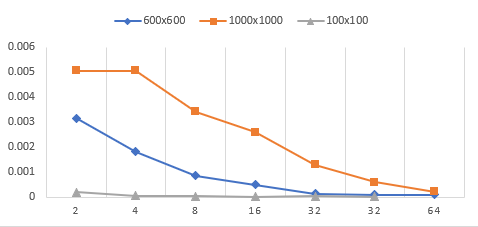
\includegraphics[height=5.5 cm\textwidth]{images/domaindecom1.png}
\caption{Time Taken for Domain Decompositions}
\end{figure}

From the figure above we can observe that for all domain sizes, as the number of cores are increased time taken to discretise the domain reduces drastically. Another point to note is that, as observed in the figure above, this effect is more pronounced for larger matrix sizes.

\vspace{-4mm}
\begin{figure}[H]
\centering
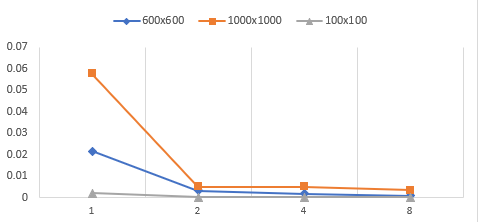
\includegraphics[height=5.5 cm\textwidth]{images/Domaindecomp2.png}
\caption{Drop in Domain Setup Time from Serial to Parallel for different Domain Sizes}
\end{figure}
An interesting point to note is the significant drop in decomposition time due to parallelisation(when we switch from one process to two), which again, is especially pronounced in larger domains.\\

\section{Affect of Domain Size and Shape on Performance}

We observe that as the domain gets more unbalanced, the \textbf{percentage of time taken for the domain decomposition} - which includes finding the number and arrangement of sub domains initialising points and memories relative to the total time is seen to reduce. The is again another feature of the kind of domain decomposition algorithm used in this code.
\vspace{-4mm}
\begin{figure}[H]
\centering
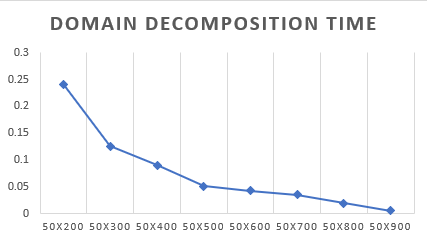
\includegraphics[height=5.5 cm\textwidth]{images/domdecomtime.png}
\caption{Drop in Domain Setup Time for a Rectangular Domain of Increasing Size}
\end{figure}
However, we ca also note that the total time taken per iteration for an increasingly rectangular domain also increases quite significantly. Upon further analysis(done in the next section) we can note this is because of the inefficiencies in MPI communications when domains are very rectangular.
\vspace{-4mm}
\begin{figure}[H]
\centering
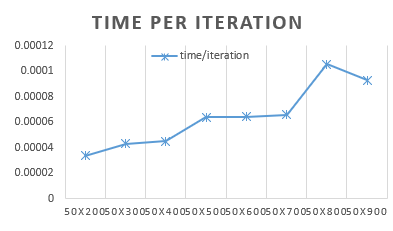
\includegraphics[height=5.5 cm\textwidth]{images/timeperiteration.png}
\caption{Time per Iteration for an Increasingly Rectangular Domain}
\end{figure}
\vspace{-4mm}
Keeping in mind the method used for domain decomposition(decompose to as close to a square as possible), we can observe some key difference in performance for two domains that have the same number of grid elements but are of different dimensions(one square and the other highly rectangular). For the sake of this analysis we assume two grids 100x100 ad 50x200 that are equal in the number of grid elements but have different shapes.\\
Consider the analysis done in the figure below comparing two domains with same number of cells but different shapes for various parameters of efficiency. We can see that on every parameter accounted for including domain setup time, MPI communications time, total iterations, and total time taken by one processor to finish the computations.
\vspace{-4mm}
\begin{figure}[H]
\centering
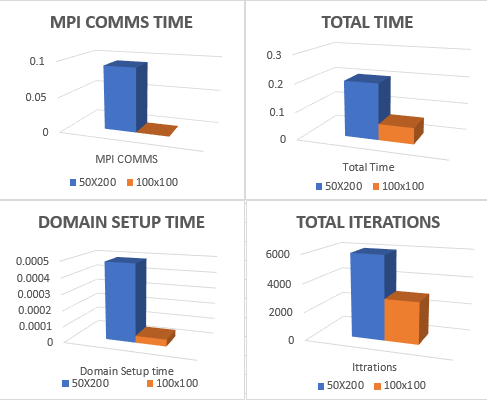
\includegraphics[height=8.3 cm\textwidth]{images/domsizeanalysis.png}
\caption{Comparison of 50x200 and 100x100 Domain Decomposition Parameters}
\end{figure}
\vspace{-4mm}

The 50x200 domain is \textbf{71.12\% less efficient in total time taken for one processor, 91.15\% slower in domain setup and almost a 100\% slower} while handling MPI communications. These calculations are based on the table below.\% Please add the following required packages to your document preamble:

\begin{table}[H]
\caption{Output Values for a 50x200 vs a 100x100 Domain}
\label{tab:my-table}
\resizebox{\columnwidth}{!}{%
\begin{tabular}{@{}lllll@{}}
\toprule
\rowcolor[HTML]{FEA966} 
\textbf{Domain Size}                     & \textbf{Total Time} & \textbf{Domain Setup Time} & \textbf{MPI Communication Time} & \textbf{Iterations} \\ \midrule
\rowcolor[HTML]{FFEAD2} 
\cellcolor[HTML]{FEA966}\textbf{50X200}  & 0.20215             & 0.000486912                & 0.092019081                     & 5971                \\
\rowcolor[HTML]{FFEAD2} 
\cellcolor[HTML]{FEA966}\textbf{100x100} & 0.0583784           & 4.31E-05                   & 1.02E-05                        & 2970                \\ \bottomrule
\end{tabular}
}
\end{table}

%----------------------------------------------------------------------------------------
\section{Efficiency of MPI Communications}

\vspace{-4mm}
\begin{figure}[H]
\centering
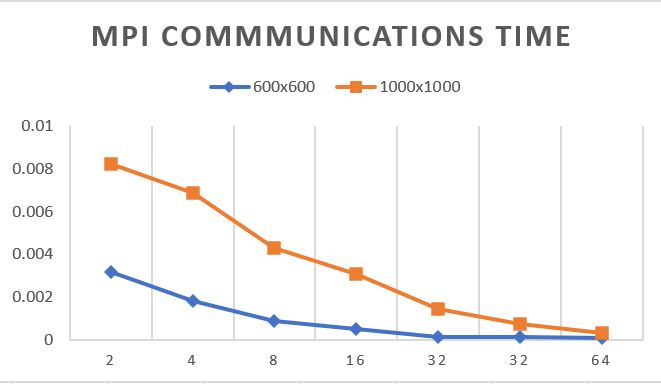
\includegraphics[height=5.5 cm\textwidth]{images/mpicomms.png}
\caption{Trends in Time Taken to complete MPI Communications for different Domain Sizes}
\end{figure}
From the figure above we see that as the number of cores used increase, the time taken for MPI communications steadily decreases. Further we can observe that for larger domain sizes the fall in MPI communication time is greater.\\
Different boundary conditions will inherently behave differently and have different setup steps to obtain correct results. For the periodic boundaries, multiple extra MPI communications with periodic neighbours are carried out. Hence, as observed in the figure 11, the time taken for periodic MPI communications on the boundaries is significantly greater.\\

\vspace{-4mm}
\begin{figure}[H]
\centering
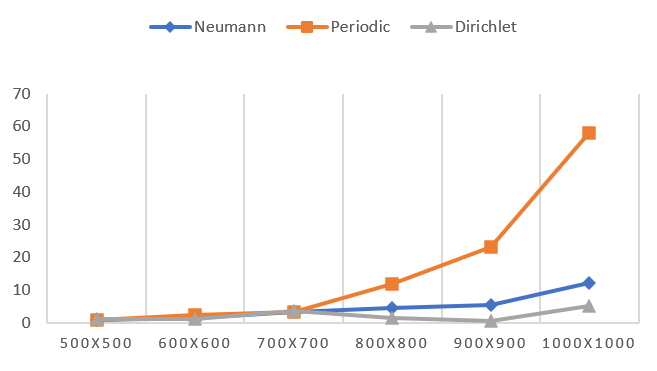
\includegraphics[height=5.5 cm\textwidth]{images/mpicomms2.png}
\caption{Comparing MPI Communication Times for Different Boundary Conditions}
\end{figure}
\vspace{-4mm}
%----------------------------------------------------------------------------------------
\section{Boundary Setup and Edge Calculation Efficiencies}
Neumann boundaries take longer to setup compared to Dirichlet since they are assigned with the values of their neighbours, whereas Dirichlet boundaries are directly set to zero, hence relatively faster.\\ 
\vspace{-4mm}
\begin{figure}[H]
\centering
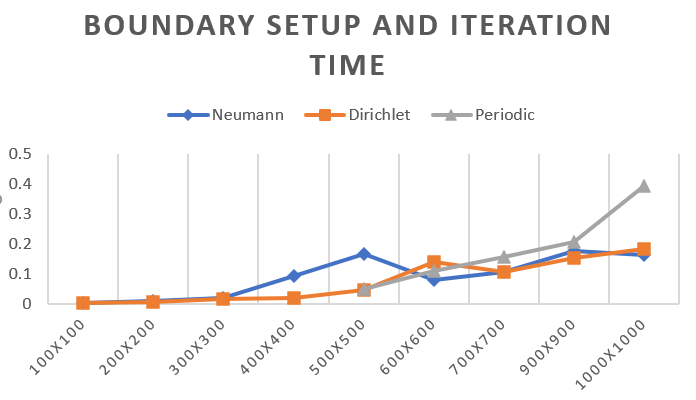
\includegraphics[height=5.5 cm\textwidth]{images/boundrysetup.png}
\caption{Boundary Setup and Edge Calculations Time}
\end{figure}
\vspace{-4mm}
While periodic boundaries have no setup times, since each processors has to engage in calculations on all sides, the total iteration time is significantly larger as observed in the figure below.\\
%----------------------------------------------------------------------------------------

\section{Selection of Cores and Nodes}
As observed in the figure below, we can see that for the same number of processes(cores), we obtain better performance if we use multiple nodes vs the same number of cores over a single node.
\vspace{-4mm}
\begin{figure}[H]
\centering
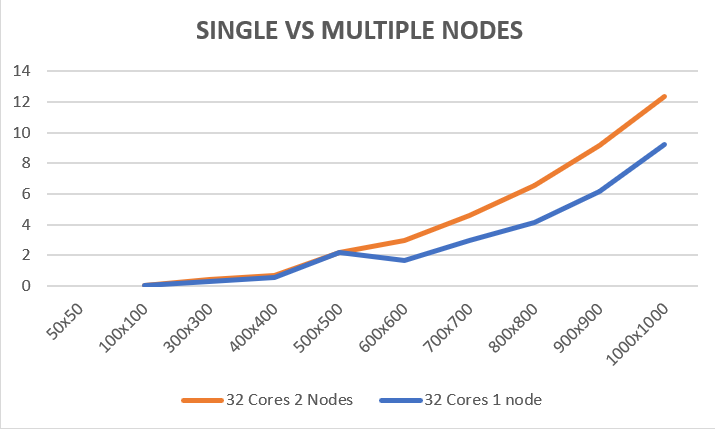
\includegraphics[height=5.5 cm\textwidth]{images/SINGLEVSMULTIPLENODES.png}
\caption{Boundary Setup and Edge Calculations Time}
\end{figure}
\vspace{-4mm}

%----------------------------------------------------------------------------------------
\section{Discussion on Further Improvements in Code}
\begin{itemize}
\item An important aspect to be further expanded upon and analysed are different types of initial disturbances. At the moment the code is setup for a single point disturbance. We could expand on this type of disturbance by creating an array of disturbance parameters to be input through the parameter file by the user. This will further allow us to study various kinds of patterns and behaviours of waves.
\item The MPI datatype class, at the moment is setup to work in the simplest most intuitive fashion by using one function that creates all the MPI data types. In order to make it more modular, we can encapsulate the creation into separate functions that can be called during creation. This will allow for further flexibility of the code.
\item In order to further ease the post-processing of data, the simulation parameters can be output into a output file that can be read into the post-processing script. This will further simply the user interface.

\end{itemize}


%----------------------------------------------------------------------------------------
%	REFERENCE LIST
%----------------------------------------------------------------------------------------
\begin{thebibliography}{99} 
\bibitem[1]{}Lecture 1 - 6: MSc ACSE - Lectures on Patterns of Parallel Programming, Prof Stephen Neethling.

 
\end{thebibliography}

%----------------------------------------------------------------------------------------

\end{document}
